\part{Types and Subtyping}

\section{Types}

\subsection{Type Systems}
\begin{definition}[Type System]
 A type system is a tractable syntactic method for
proving absence of certain program behaviors by
classifying phrases according to the kinds of values
they compute.
\end{definition}
\begin{description}
 \item[Syntactic] Rules are based on form, not behavior
 \item[Phrases] Expressions, methods, etc... of a program. 
 \item[Kinds of values] Types
\end{description}

\subsection{Weak and Strong Type Systems}
\begin{description}
 \item[Untyped Languages] Do not classify values into types.\\
  Example: Assembler
 \item[Weakly-typed Languages] Classify values into types, but do not srictly enforce additional restrictions.\\
  Examples: C, C++
 \item[Strongly-typed Languages] Enforce that all operations are applied to arguments of the appropriate types.\\
  Examples: C\#, Eiffel, Java, Python, Scala, Smalltalk
\end{description}

Strongly-typed languages prevent certain
erroneous or undesirable program behavior
Comparison between strong and weak typing:
\lstset{language=C}
\begin{lstlisting}[caption=C Example]
int main( int argc, char** argv ) { 
  int i = ( int ) argv[ 0 ]; 
  printf( "%d", i ); 
} 
\end{lstlisting}
\lstset{language=Java}
\begin{lstlisting}[caption=Java Example]
int main( String[ ] argv ) {
  int i = ( int ) argv[ 0 ];
  System.out.println( i );
}
\end{lstlisting}
The Java example results in a Compile-time error.

\subsection{Types}
\begin{definition}[Types]
A type is a set of values sharing some properties. A value v has type T if v is an element of type. 
\end{definition}
\begin{description}
 \item[Nominal Types] are based on \emph{type names}\\
  Examples: C++, Eiffel, Java, Scala
 \item[Structural Types] are based on \emph{availability of methods and fields}\\
 Examples: Python, Ruby, Smalltalk
\end{description}
\subsubsection{Example}

\lstset{language=C}
\begin{lstlisting}
class S {
  m( int ) { ... }
  n( )     { ... }
}

class T {
  m( int ) { ... }
  n( )     { ... }
}
\end{lstlisting}
\begin{itemize}
 \item \textbf S and \textbf T are \emph{\textbf{different} in nominal systems}
 \item \textbf S and \textbf T are \emph{\textbf{equivalent} in structural systems}
\end{itemize}

\subsection{Static Type Checking}
\emph{Each expression} of a program \emph{has a type}. \emph{Types} of variables and methods are \emph{declared explicitly} or \emph{inferred}. Types of expressions can be derived from the types of their constituents. \emph{Type rules} are used \emph{at compile time} to check whether a program is \emph{correctly typed}.
\paragraph{Examples: } $\text{}$
\begin{lstlisting}[caption=compiles]
int a;
boolean equals(Object o)
a + 7
"A number: " + 7
"A string".equals(null)
\end{lstlisting}
\begin{lstlisting}[caption=results in compile-time errors]
a = "A string";           // Assignment of a String to an integer
"A string".equals(1, 2);  // Too many arguments
\end{lstlisting}

\subsection{Dynamic Type Checking}
\emph{Variables}, \emph{methods}, and \emph{expressions} of a program \emph{are} typically \emph{not typed}. Every object and value has a type. A \emph{Run-time system} checks that operations are applied to \emph{expected arguments}.

\subsection{Static Type Safety}
\begin{definition}[Static Type Safety]
 A programming language is called type-safe if its design prevents type errors. 
\end{definition}
% Statically type-safe object-oriented languages
% \paragraph{Guarantees}: Statically type-safe object oriented languages guarantee the following invariant:
\begin{shadequote}
 In every execution state, the type of the value held by variable v is a subtype of the declared type of v.
\end{shadequote}
Most static type systems rely on dynamic checks for certain operations. Such as \emph{type conversion by casts}. \emph{Run-time checks} throw an exception in case of a type error.

\begin{lstlisting}[caption=Java example on a dynamic check]
Object[] oa = new Object[10];
String s    = "A String";
oa[0]       = s;
// ..
if (oa[0] instanceof String) {
  s = (String) oa[0];
}
s = s.concat("Another String");
\end{lstlisting}

Static checkers need to \emph{approximate run-time behavior} (conservative check). 
\lstset{language=Python}
\begin{lstlisting}[caption=Python example on dynamic type checking]
def divide(n,d):
  if d != 0:
    res = n/d
  else:
    res = "Division by zero"
  print res
\end{lstlisting}

Dynamic checkers support \emph{on-the-fly code generation} and dynamic class loading.
\lstset{language=Java}
\begin{lstlisting}[caption=JavaScript example on on-the-fly code generation]
eval (
  "x=10; y=20; document.write(x*y);"
);
\end{lstlisting}

\subsection{Comparison}

\subsection{Advantages of static checking}
\begin{description}
 \item[Static safety:] More errors are found at compile time.
 \item[Readability:] Types are excellent documentation.
 \item[Efficiency:] Type information allows optimizations.
\end{description}
\subsection{Advantages of dynamic checking}
\begin{description}
 \item[Expressiveness:] No correct program is reject by the type checker.
 \item[Low overhead:] No need to write type annotations.
 \item[Simplicity:] Static type systems are often complicated.
\end{description}

\begin{tabular}{r|p{5cm}p{5cm}}
& \textbf{Static} & \textbf{Dynamic}\\ \hline
\textbf{Nominal} & C++, C\#, Eiffel, Java, Scala & For certain features of statically-typed languages.\\
\textbf{Structural}& Research languages such as Moby, PolyToil, O'Caml. & JavaScript, Python, Ruby, Smalltalk.
\end{tabular}\\

Dynamically typed languages with a structural types are also called \emph{duck typed languages}.

\section{Subtyping}

\begin{shadequote}
  Objects of subtypes can be used wherever objects of supertypes are expected.\par\emph{Substitution principle}
\end{shadequote}

\begin{description}
 \item[Syntactic classification] Subtype objects can \emph{understand at least the messages} that supertype objects can understand.
 \item[Semantic classification] Subtype objects \emph{provide at least the behavior} of supertype objects.
\end{description}

The \emph{subtype relation} corresponds to the \emph{subset relation} on the values of a type.
\begin{figure}[h!]
  \centering
    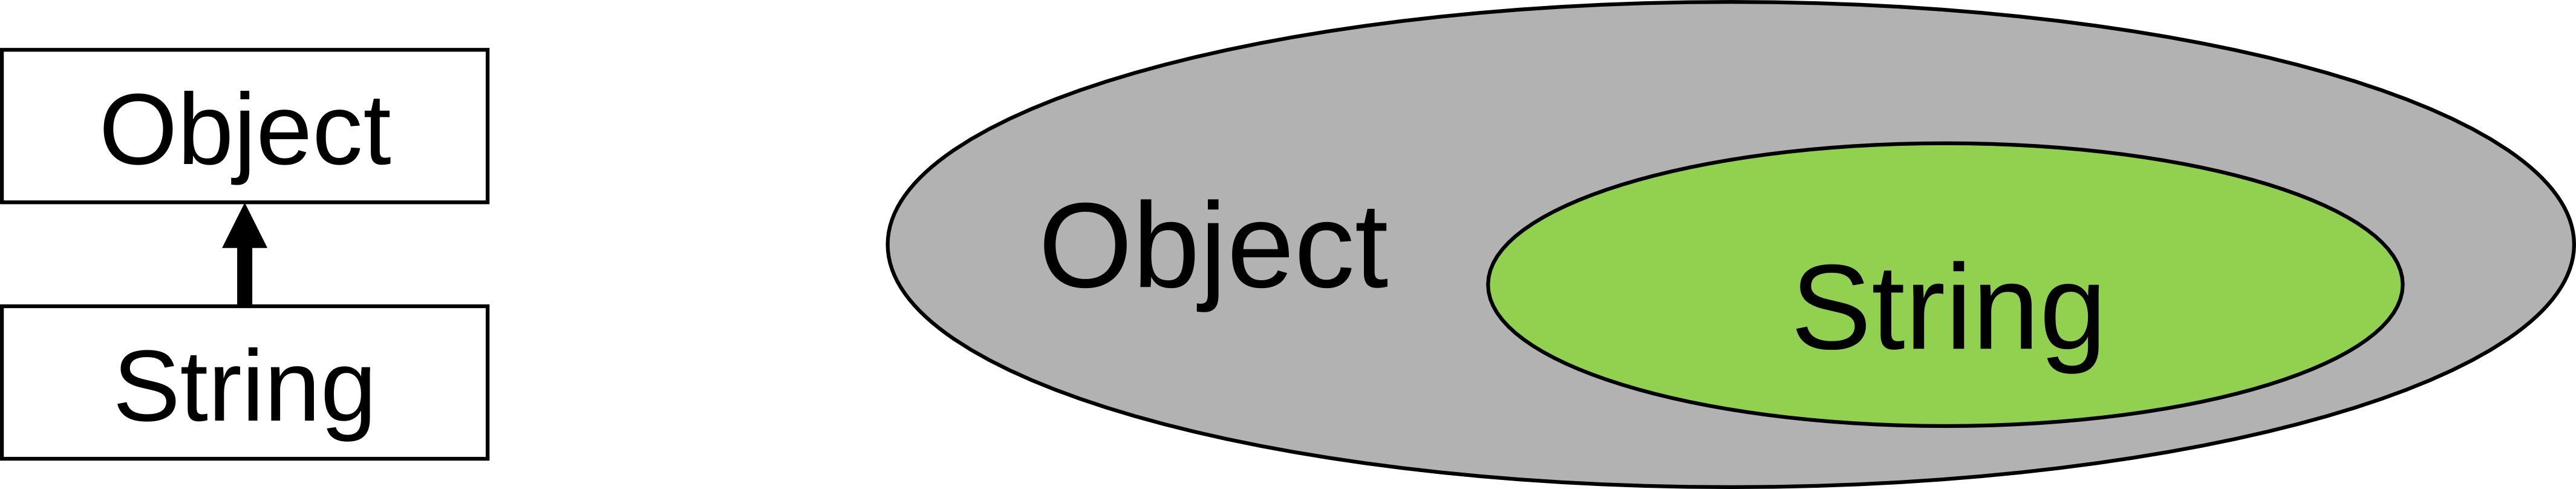
\includegraphics[width=0.5\textwidth]{img/02_subtype_relation}
%       \caption{Core Requirements in Software Technology}
\end{figure}

\begin{description}
 \item[Nominal type systems] Determine \emph{type membership} based on \emph{type names} and determine \emph{subtype relations} based on \emph{explicit declarations}:
 \lstset{language=Java}
 \begin{lstlisting}[caption=nominally typed language]
  class S { 
    m(int) {...} 
  }
  class T extends S { // nominal subtype because of extend declaration
    m(int) {...} 
  }
  class U {           // not a subtype of S
    m(int) {...}
    n()    {...}
  }
 \end{lstlisting}
  \item[Structural type systems] Determine \emph{type membership} and \emph{subtype relations} based on \emph{availability of methods and fields}:
  \begin{lstlisting}[caption=structurally typed language]
  class S {
    m(int) {...]
  }
  class T {         // Subtype of S
    m(int) {...}
  }
  class U {         // Subtype of U
    m(int) {...}
    n()    {...}
  }
  \end{lstlisting}

\end{description}

\subsection{Nominal Subtyping and Substitution}
Subtype objects can \emph{understand at least the messages} that supertype objects can understand:
\begin{itemize}
 \item Method calls
 \item Field accesses
\end{itemize}
Subtype objects have \emph{wider interfaces} than supertype objects:
\begin{itemize}
 \item Existence of methods and fields
 \item Accessibility of methods and fields
 \item Types of methods and fields
\end{itemize}

\subsubsection{Rules}
\begin{description}
 \item[Existence] \emph{Subtypes may add, but not remove methods and fields}
 \item[Accessibility] An \emph{overriding method must not be less accessible} than the methods it overrides:
 \begin{lstlisting}
  class Super {
    public void foo() {...}
    public void bar() {...}
  }
  
  class Sub <: Super {
    public void foo() {...}
    private void bar() {...} 
  }
  
  void m( Super s) { s.bar(); }
 \end{lstlisting}
 At run time, \lstinline{m} could access a private method of \lstinline{Sub}, thereby violating information hiding.
 \item[Contravariant parameters] An \emph{overriding method must not require \textbf{more specific} parameter types} than the method it overrides.
 \item[Covariant results] An \emph{overriding method must not have \textbf{more genera} result type} than then the ethod it overrides. 
\end{description}

